%%
%%   Version 3.1 of 16 May 2019.
%%

\usepackage{graphicx}% Include figure files
\usepackage{dcolumn}% Align table columns on decimal point
\usepackage{bm}% bold math

% hyphenation
\usepackage{hyphenat}

% tables
\usepackage{multirow}
\usepackage{booktabs}

% mathematics
\usepackage{amsmath}
\usepackage{amsfonts}
\usepackage{amssymb}
\usepackage{amsbsy}
\usepackage{mathrsfs}
\usepackage{upgreek}
\usepackage[cbgreek]{textgreek}

%---------------------------------------------------
% Approximations
\newcommand{\Approx}[2]{\ensuremath{\text{Ap}_{#2} \left[ {#1} \right] }}
% happy integral
\newcommand{\rint}[1]{\mbox{\Large $ \int\limits_{\mbox{\tiny  $#1$}}$}}
% SHORTCUTS
%\newcolumntype{,}{D{.}{,}{2}}
\newcommand{\citee}[1]{\ensuremath{\scriptsize^{\citenum{#1}}}}
\newcommand{\HRule}{\rule{\linewidth}{0.2mm}}
% Quantum notation
\newcommand{\Bra}[1]{\ensuremath{\bigl\langle {#1} \bigl\lvert}}
\newcommand{\Ket}[1]{\ensuremath{\bigr\rvert {#1} \bigr\rangle}}
\newcommand{\BraKet}[2]{\ensuremath{\bigl\langle {#1} \bigl\lvert {#2} \bigr\rangle}}
\newcommand{\tBraKet}[3]{\ensuremath{\bigl\langle {#1} \bigl\lvert {#2} \bigl\lvert {#3} \bigr\rangle}}
%
\newcommand{\bra}[1]{\ensuremath{\bigl( {#1} \bigl\lvert}}
\newcommand{\ket}[1]{\ensuremath{\bigr\rvert {#1} \bigr)}}
\newcommand{\braket}[2]{\ensuremath{\bigl( {#1} \bigl\lvert {#2} \bigr)}}
\newcommand{\tbraket}[3]{\ensuremath{\bigl( {#1} \bigl\lvert {#2} \bigl\lvert {#3} \bigr)}}
% Math
\newcommand{\pd}{\ensuremath{\partial}}
\newcommand{\DR}{\ensuremath{{\rm d} {\bf r}}}
%\newcommand{\BM}[1]{\ensuremath{\mbox{\boldmath${#1}$}}}
\newcommand{\BM}[1]{\bm{#1}}
% Chemistry (formulas)
\newcommand{\ch}[2]{\ensuremath{\mathrm{#1}_{#2}}}
% Math 
\newcommand{\VEC}[1]{\ensuremath{\mathrm{\mathbf{#1}}}}
% vector nabla
\newcommand{\Nabla}{\ensuremath{ \BM{\nabla}}}
% derivative
\newcommand{\FDer}[3]{\ensuremath{
\bigg(
\frac{\partial #1}{\partial #2}
\bigg)_{#3}}}
% diagonal second derivative
\newcommand{\SDer}[3]{\ensuremath{
\biggl(
\frac{\partial^2 #1}{\partial #2^2}
\biggr)_{#3}}}
% off-diagonal second derivative
\newcommand{\SSDer}[4]{\ensuremath{
\biggl(
\frac{\partial^2 #1}{\partial #2 \partial #3}
\biggr)_{#4}}}
% derivatives without bound
% derivative
\newcommand{\fderiv}[2]{\ensuremath{
\frac{\partial #1}{\partial #2}}}
% diagonal second derivative
\newcommand{\sderiv}[2]{\ensuremath{
\frac{\partial^2 #1}{\partial #2^2}
}}
% off-diagonal second derivative
\newcommand{\sderivd}[3]{\ensuremath{
\frac{\partial^2 #1}{\partial #2 \partial #3}
}}
% derivatives for tables
\newcommand{\fderivm}[2]{\ensuremath{
{\partial #1}/{\partial #2}}}
% diagonal second derivative
\newcommand{\sderivm}[2]{\ensuremath{
{\partial^2 #1}/{\partial #2^2}
}}
% off-diagonal second derivative
\newcommand{\sderivdm}[3]{\ensuremath{
{\partial^2 #1}/{\partial #2 \partial #3}
}}
% ERIs and OEIs
\newcommand{\OEIc}[3]{\ensuremath{\left(#1 \lvert #2 \rvert #3 \right)}}
\newcommand{\ERIc}[4]{\ensuremath{\left(#1 #2 \vert #3 #4 \right)}}

% Partial density and potential
\newcommand{\PartPot}[4]{\ensuremath{\frac{#1 #2}{\lvert #3-#4 \rvert }}}

% trace operator
\DeclareMathOperator{\Tr}{Tr}

%\draft % marks overfull lines with a black rule on the right

% Define location of graphics
\graphicspath{{./figures/}}

\begin{document}
\preprint{AIP/123-OEP}

\title{Ab Initio Effective One-Electron Potential Operators:
Applications for Charge-Transfer Energy in Effective Fragment Potentials}

\author{Bartosz B{\l}asiak}
\email[]{blasiak.bartosz@gmail.com}
\homepage[]{https://www.polonez.pwr.edu.pl}

\author{Marta Cho{\l}uj} 
\author{Joanna D. Bednarska}
\author{Wojciech Bartkowiak}

\affiliation{Department of Physical and Quantum Chemistry, Faculty of Chemistry, 
Wroc{\l}aw University of Science and Technology, 
Wybrze{\.z}e Wyspia{\'n}skiego 27, Wroc{\l}aw 50-370, Poland}

\date{\today}

\begin{abstract}
The concept of the effective one-electron potentials has been useful for many decades
in efficient description of electronic structure of chemical systems, especially extended
molecular aggregates such as interacting molecules in condensed phases.
\end{abstract}

\pacs{}

\maketitle

\tableofcontents

\section{\label{ss.5.2}Introduction}

Charge transfer (CT) between molecules occurs when the net electronic populations 
of interacting molecules change which leads to an additional stabilization 
of a molecular aggregate. The effect of CT on the interaction energy 
is known to be often non\hyp{}negligible, especially
in donor\hyp{}acceptor systems such as H\hyp{}bonded species
and charged complexes.
\emph{Ab initio} fragmentation methods, such as
the second generation of the effective fragment potential method (EFP2),
are often used to describe the homogeneous extended molecular systems 
such as solutions
and recently even biomolecules. EFP2 relies on the intermolecular 
perturbation theory, and the total interaction energy is approximated as
a sum of five contributions due to the Coulombic interaction of the unperturbed (isolated)
charge densities of the monomers, exchange\hyp{}repulsion energy,
induction energy due to mutual polarization, intermolecular dispersion energy,
as well as the CT energy,
%
\begin{equation}
 U^{\rm EFP2} \approx U^{\rm Coul} + U^{\rm Ex-Rep} + U^{\rm Ind} + U^{\rm Disp} + U^{\rm CT} \;.
\end{equation}
%
However, calculating the CT stabilization energy is usually much more expensive 
than evaluating the contributions due to other effects.\cite{Gordon.Fedorov.Pruitt.Slipchenko.ChemRev.2012}
%However, the computational cost of the CT term is usually at least few times larger
%than the next costly contribution $U^{\rm Ex-Rep}$, which is still too costly
%to perform molecular dynamics (MD) simulations including the $U^{\rm CT}$. 
In effect,
this part of the EFP2 energy is usually ignored in most of the applications. In the 
recent LIBEFP library, CT term were even not implemented due to those reasons.

In this work, we propose an alternative formulation of the CT energy compatible with the
EFP2 method. We start from the perturbation theory of Murrell et al.
and
introduce the effective one\hyp{}electron potential (OEP) operators
to eliminate the electron\hyp{}repulsion integrals (ERI's) from the original theory.
Later we validate the model against the EFP2 method in Section XXX. Finally,
we conclude this work and provide few remarks on future development in Section XXX.

\section{\label{s:2}Effective One-Electron Potential Operators}

To establish the notation within the present work, 
the formalism of one\hyp{}electron potential (OEP) operators is
given first.
The one\hyp{}electron Coulomb static effective potential $v^{\rm eff}({\bf r})$
produced by a certain effective one\hyp{}electron charge density distribution $\rho^{\rm eff}({\bf r})$
is 
%
\begin{equation} \label{e:v-eff}
	v^{\rm eff}({\bf r}) = \int \frac{ \rho^{\rm eff}({\bf r}') }{ \vert {\bf r}' - {\bf r} \vert} d{\bf r}' \;,
\end{equation}
%
where ${\bf r}$ is a spatial coordinate. 
For convenience, the total effective density can be split into nuclear and electronic contributions,
%
\begin{equation} \label{e:rho-eff}
 \rho^{\rm eff}({\bf r}) = \lambda \rho^{\rm eff}_{\rm nuc}({\bf r}) + \rho^{\rm eff}_{\rm el}({\bf r}) \;,
\end{equation}
%
where $\lambda$ is a certain parameter and is assumed either 1 or 0 in this work.
Formally, the electronic part can be expanded in terms of an effective
one\hyp{}particle density matrix represented in a certain basis of orbitals, $\BM{\phi}({\bf r})$,
%
\begin{equation} \label{e:d-spectral}
	\rho^{\rm eff}_{\rm el}({\bf r}) = \sum_{\alpha\beta} D_{\alpha\beta}^{\rm eff} 
	\phi_\alpha({\bf r}) \phi_\beta^{*}({\bf r})  \;.
\end{equation}
%
Based on that, the operator form of the effective potential 
can be written as
%
\begin{equation} \label{e:oep-operator}
	\hat{v}^{\rm eff} = 
        \lambda \hat{v}_{\rm nuc} +
        %\sum_{\alpha\beta} 
	%\Ket{\alpha} 
        \int d{\bf r} \Ket{{\bf r}} 
        v^{\rm eff}({\bf r})
	%\left[
	%\int
	%\hat{J}^{\rm}_{\alpha\beta}({\bf r}') 
	%\rho^{\rm eff}({\bf r}')
	%d{\bf r}' 
	%\right]
	%\Bra{\beta}  
        \Bra{{\bf r}}
\end{equation}
%
with the nuclear
%and Coulomb operators 
operator
defined by
%
%\begin{subequations}
%\begin{align}
\begin{equation}
        \hat{v}_{\rm nuc} \equiv \sum_x^{\rm At}  
                     \int d{\bf r} \Ket{{\bf r}} 
                     \frac{Z_x}{\vert {\bf r} - {\bf r}_x \vert}
                     \Bra{{\bf r}} \;.
	%\hat{J}^{\rm}_{\alpha\beta}({\bf r}) f({\bf r}) &\equiv
	%f({\bf r}) 
	%\int
	%\frac{ \phi_\alpha^{*}({\bf r}') \phi_\beta({\bf r}') }{ \vert {\bf r}' - {\bf r} \vert} d{\bf r}'
\end{equation}
%\end{align}
%\end{subequations}
%
%for any one\hyp{}electron function $f({\bf r})$. 
and $\BraKet{\bf r}{\alpha} = \varphi_\alpha({\bf r})$.
The matrix element of the effective potential operator
is therefore given by
%
\begin{equation}
	\tBraKet{\alpha}{ \hat{v}^{\rm eff} }{\beta}
	= \lambda \sum_x^{\rm At} W_{\alpha\beta}^{(x)} +
        \sum_{\gamma\delta} \BraKet{\alpha\beta}{\gamma\delta} D^{\rm eff}_{\gamma\delta}  \;,
\end{equation}
%
where 
%
\begin{equation}
 W_{\alpha\beta}^{(x)} = 
 Z_x \int \frac{\phi^*_\alpha({\bf r}) \phi_\beta({\bf r})}{\vert {\bf r} - {\bf r}_x \vert} d{\bf r} \;,
\end{equation}
%
$Z_x$ is the atomic number of the $x$th atom,
and the symbol `At' denotes all atoms that contribute to the effective potential.
In the above equation and throughout the work, 
%
\begin{equation}
\tBraKet{\alpha}{\mathscr{O}(1)}{\beta} \equiv \int \phi^*_\alpha({\bf r}) \mathscr{O}(1) \phi_\beta({\bf r}) d{\bf r} 
\end{equation}
%
for any one\hyp{}electron operator $\mathscr{O}(1)$ 
and the electron repulsion integral (ERI)
is defined according to
%
\begin{equation}
	\BraKet{\alpha\beta}{\gamma\delta} \equiv
	\iint 
	\frac{ \phi_\alpha^{*}({\bf r}_1) \phi_\beta({\bf r}_1) 
	       \phi_\gamma^{*}({\bf r}_2) \phi_\delta({\bf r}_2) }{ \vert {\bf r}_1 - {\bf r}_2 \vert}
	d{\bf r}_1 d{\bf r}_2  \;.
\end{equation}
%

%\subsection{\label{s.334}Practical OEP-Based Calculations}

\subsection{\label{ss:2.3}Incorporating Electron Repulsion Integrals into Effective Potentials}

Consider now an arbirtary functional $\mathcal{F}$ that explicitly depends on the 
ERI's. In this work, OEP's are defined by the following transformation
%
 \begin{equation}
 \mathcal{F}
 \left[ 
   \BraKet{ij}{k^Al^A}
	 \right] = \tBraKet{i}{\hat{v}_{kl}^A}{j}  \;,
 \end{equation}
%
where 
% $A$ and $B$ denote different molecules and $\phi_i$ is the $i$th molecular orbital
%or basis function.
$\hat{v}_{kl}^A$ is the effective one-electron potential operator given by Eq.~\eqref{e:oep-operator} 
with the
effective density $\rho_{kl}^A({\bf r}) \equiv \phi_k^A({\bf r})\phi_l^A({\bf r})$.
The summations over $k$ and $l$ can be incorporated into the total effective one-electron potential operator
$\hat{v}_{\text{eff}}^A$
to produce
%
\begin{equation}
	\sum_{ij}\sum_{kl\in A} \mathcal{F}\left[ 
   \BraKet{ij}{k^Al^A}
 \right] = \sum_{ij} \tBraKet{i}{\hat{v}_{\text{eff}}^A}{j}  \;.
\end{equation}
%
Thus, the total computational effort is, in principle, reduced from the fourth-fold
sum involving evaluation of ERI's to the two-fold sums of cheaper one-electron integrals.
It is also possible to generalize the above expression even further by
summing over all possible functionals ${\mathcal{F}}_t$
%
\begin{equation} \label{e:ft-reduction}
	\sum_t \sum_{ij}\sum_{kl\in A} {\mathcal{F}}_t\left[ 
   \BraKet{ij}{k^Al^A}
 \right] = \sum_{ij} \tBraKet{i}{\hat{v}_{\text{eff}}^A}{j} \;.
\end{equation}
%
The above design has the advantage that it opens the possibility to define first\hyp{}principles
effective fragments as long as the $P_{ij}$ and $P_{ijkl}$ 
from Eq.~\eqref{e:exp-val-series} are computable and can be approximately
partitioned in between the interacting fragments.
%the resulting effective potentials are fully first\hyp{}principles
%and no extensive case\hyp{}dependent fitting procedures are necessary as long as the $P_{ij}$ and $P_{ijkl}$
%are computable.
%Only the effective potentials of \emph{independent} fragment $A$ need to be determined once and for all
%and stored in a file. 
%Note also, that, in principle, there is no approximation 
%made here at that moment.



Two general cases of basis function partitioning scheme
are considered in this work,
in which it is possible to define an effective one\hyp{}electron
potential. They are listed in Table~\ref{t:oep-matrix-element-types}.
The first type is a Coulomb\hyp{}like contribution, for which multipole expansion or density fitting can be used.
The second type is an overlap\hyp{}like contribution, which can be approximated via the density fitting. 
%
{
\renewcommand{\arraystretch}{1.4}
\begin{table}[b]
\caption[Types of matrix elements with OEP operators]
{{\bf Types of matrix elements with OEP operators\footnotemark[1]}
}
\label{t:oep-matrix-element-types}
\begin{ruledtabular}
\begin{tabular}{lcccc}
Matrix element      &&            `Overlap-like'                &&            `Coulomb-like'               \\ 
                    && $\tBraKet{i}{\hat{v}^{A}_{\rm eff}}{j} $ && $\tBraKet{j}{\hat{v}^{A}_{\rm eff}}{l}$ \\ 
	\cline{1-5}
Partitioning scheme &&            $i\in A, j\in B$              &&               $j,l\in B$                \\
Associated ERI's    &&            $\BraKet{AA}{AB}$             &&               $\BraKet{AA}{BB}$         \\
DF\footnotemark[2]/RI\footnotemark[3] Form    
&& $\sum_{\xi\in A}^{\rm Aux} v^A_{i\xi} S^{AB}_{\xi j} $  
&& $\sum_{\xi\zeta\in A}^{\rm Aux} S^{BA}_{j\xi} v^A_{\xi\zeta} S^{AB}_{\zeta l} $ \\
DMTP\footnotemark[4] Form                     
&& --  &  &  $\rho_{jl}^B \odot \rho_{\rm eff}^A$ \\
\end{tabular}
\end{ruledtabular}
%
\footnotetext[1]{Test footnotemark.}
\footnotetext[2]{Density Fitting}
\footnotetext[3]{Resolution of Identity}
\footnotetext[4]{Distributed Multipole Expansion}
%
\end{table}
}
%

\subsection{\label{s.333}Distributed Multipole Expansion of OEP's}

This scheme is most applicable in the case of matrix elements of the type
$
 \tBraKet{j^B}{\hat{v}_{\rm eff}^A}{l^B}
$
because it can be considered as a Coulombic interaction between $\rho^B_{jl}$
and $\rho^A_{\rm eff}$. 
In general, given certain two effective one\hyp{}electron density distributions,
the associated effective Coulombic interaction energy can be estimated from the classical formula
according to
%
\begin{equation}
 \Delta^{(XY)}_{\rm eff} E_{\rm Coul} = \iint \frac{\rho_{\rm eff}^X({\bf r}_1) \rho_{\rm eff}^Y({\bf r}_2)}
 {\vert {\bf r}_1 - {\bf r}_2 \vert} 
d{\bf r}_1 d{\bf r}_2 \;.
\end{equation}
%
The above integral can be approximated by the
distributed multipole (DMTP)
expansions of the respective densities as follows
%
\begin{multline}
  \Delta^{(XY)}_{\rm eff} E_{\rm Coul} \approx
 \rho_{\rm eff}^X \odot \rho_{\rm eff}^Y \equiv
 \sum_{u\in A} \sum_{w\in B} \Big\{ 
 T^{(0)}_{uw}
 q_{\rm eff}^{(u)}  q_{\rm eff}^{(w)} \\
 - {\bf T}^{(1)}_{uw} \cdot 
   \left[ q_{\rm eff}^{(u)} {\BM\upmu}_{\rm eff}^{(w)} - q_{\rm eff}^{(w)} {\BM\upmu}_{\rm eff}^{(u)} \right]
 - {\bf T}^{(2)}_{uw} : 
  {\BM\upmu}_{\rm eff}^{(u)}  \otimes {\BM\upmu}_{\rm eff}^{(w)} 
 \ldots
 \Big\}
\end{multline}
%
In the above equations, $q_{\rm eff}^{(u)}$ and ${\BM\upmu}^{(u)}_{\rm eff}$ 
are the effective distributed monopole (charge)
and dipole moment, respectively, centered on the $u$th site, 
whereas ${{\bf T}^{(r)}_{uw}}$ are the so called interaction tensors or rank $r$ 
that can be found elsewhere.
The symbol `$\odot$' denotes the sum of all the tensor contractions
performed over the DMTP's of molecule $X$ and $Y$ to yield the associated interaction energy.
The choice of the distribution centres as well as the truncation order of the multipole expansion
is crucial in compromising the accuracy and computational cost of the resulting expressions.
There is many ways in which this can be achieved, e.g., through the distributed multipole analysis (DMA)
of Stone and Anderton, %cite
the cumulative atomic multipole moments of Sokalski and Poirier, %cite
the localised distributed multipole expansion (LMTP) of Etchtebest et al. %cite
or schemes based on fitting to electrostatic potential.

\subsection{\label{s.3344}Density Fitting of OEP's}

This scheme is most useful in the case of matrix elements of the type
$
 \tBraKet{i^A}{\hat{v}_{\rm eff}^A}{j^B}
$.
To get the \emph{ab initio} representation of such an overlap\hyp{}like matrix element,
one can use a procedure similar to
the typical density fitting or resolution of identity, both of which are nowadays widely used 
to compute electron\hyp{}repulsion integrals (ERI's) more efficiently. 

\subsubsection{Density Fitting in Nearly-Complete Space}

An arbitrary one\hyp{}electron potential of molecule $A$ acting on any state vector 
associated with molecule $A$ can be expanded in an auxiliary space centered 
on $A$ as
%
\begin{equation}
   \hat{v}^{A}\Ket{i} = \sum_{\xi\eta}^{\rm RI} \hat{v}^{A}\Ket{\xi} [{\bf S}^{-1}]_{\xi\eta} \BraKet{\eta}{i}
\end{equation}
%
under the necessary assumption that the auxiliary basis set is nearly complete,
i.e., 
$\sum_{\xi\eta}^{\rm RI} \Ket{\xi}[{\bf S}^{-1}]_{\xi\eta} \Bra{\eta} \cong 1$.
In the equations above, 
the `RI' symbol denotes a certain auxiliary basis set that fulfills the resolution of identity. 
%In a special case when the basis set is orthogonal (e.g., molecular orbitals)
%the above relation simplifies to
%\begin{equation}
%   v\vert i) = \sum_{\xi} v\vert \xi) ( \xi \vert i)
%\end{equation}
Such a general expansion can be obtained by 
utilizing the density fitting
in the nearly\hyp{}complete space,
%
\begin{equation}
 \hat{v}^{A}\Ket{i} = \sum_{\xi}^{\rm RI} V^A_{i\xi} \Ket{\xi} \;.
\end{equation}
%
In the above equation,
the matrix ${\bf V}^A$
is the projection of the state vector $\hat{v}^{A} \Ket{i}$
onto the complete basis $\{ \varphi_\xi \}$.
Let $Z_i[{\bf V}^A]$ be the least\hyp{}squares objective function 
%
\begin{equation} \label{e:z-compl}
 Z_i[{\bf V}^A] = \int \vert \Xi_i({\bf r}) \vert^2 d{\bf r}
\end{equation}
%
with the error density defined by
%
\begin{equation}
 \Xi_i({\bf r}) = v^A({\bf r}) \phi_i({\bf r}) - \sum_\xi^{\rm RI} V^A_{i\xi} \varphi_\xi({\bf r}) \;.
\end{equation}
%
By requiring that
%
\begin{equation} \label{e:z-necessary-requirement}
 \frac{\partial Z_i[{\bf V}^A]}{\partial V^A_{i\mu}} = 0 \text{ for all $\mu$}
\end{equation}
%
one finds the coefficients of the $i$th row of ${\bf V}^A$ to be
%
\begin{equation} \label{e:gdf-coml.v}
% {\bf v}_i = {\bf a}^{(i)} \cdot {\bf S}^{-1}
  V^A_{i\xi} = \sum_\eta^{\rm RI} [{\bf S}^{-1}]_{\xi\eta} a^{(i)}_\eta \;,
\end{equation}
%
where the auxiliary matrices are given by
%
\begin{subequations}
\begin{align}
 a^{(i)}_\eta &= \int \varphi^*_\eta({\bf r}) \hat{v}^A \phi_i({\bf r}) d{\bf r} \;,\\  
 S_{\eta\xi}  &= \int \varphi^*_\eta({\bf r}) \varphi_\xi({\bf r}) d{\bf r} \;.
\end{align}
\end{subequations}
%
%Since matrix elements of an OEP operator in auxiliary space can be computed 
%in the same way as the matrix elements with any other basis function, 
%one can formally write the following identity
%\begin{equation}
% (X \vert v\vert i) = \sum_{\xi\eta} S_{X \xi} [{\bf S}^{-1}]_{\xi\eta} (\eta\vert v\vert i)
%\end{equation}
%where $ X $ is an arbitrary orbital.
%When the other orbital
%does not belong to molecule $A$ but to the (changing) environment, it is 
%straightforward to compute the resulting matrix element, which is simply given as  
%\begin{equation}
%   (j_{\in B} \vert v^A \vert i_{\in A}) = \sum_\xi {S_{j\xi}} {G_{i\xi}}
%\end{equation}
%where $j$ denotes the other (environmental) basis function.
%
The working formula for $a^{(i)}_\eta$ can be found by applying 
potential form from Eq.~\eqref{e:v-eff}
along with the spectral representation of the effective density from Eq.~\eqref{e:d-spectral} 
which finally gives
%
\begin{equation}
 a^{(i)}_\eta = \lambda \sum_{x} W_{\eta i}^{(x)} + 
 \sum_{\alpha\beta} D^A_{\alpha\beta} 
  \BraKet{\alpha\beta}{\eta i} \;.
%  \iint \frac{ \phi_\alpha^*({\bf r}_1)  \phi_\beta({\bf r}_1) \varphi^*_\eta({\bf r}_2) \phi_i({\bf r}_2)}
% {\vert {\bf r}_1 - {\bf r}_2 \vert }
% d{\bf r}_1 d{\bf r}_2
\end{equation}
%

\subsubsection{Density Fitting in Incomplete Space}

Density fitting scheme from previous section has practical disadvantage of a nearly\hyp{}complete basis set
being usually very large (spanned by large amount of basis set vectors). 
Since most of basis sets used in quantum chemistry do not form a nealy complete
set, it is beneficial to design a modified scheme in which it is possible to obtain the effective 
matrix elements of the OEP operator in a incomplete auxiliary space. This can be achieved by minimizing 
the following objective function
%
\begin{equation} \label{e:z-incompl}
	Z_i[{\bf V}^A] = \iint 
        \frac{ \Xi_i^*({\bf r}_1) \Xi_i({\bf r}_2) }{\vert {\bf r}_1 - {\bf r}_2 \vert}  
         d{\bf r}_1 d{\bf r}_2  \;.
\end{equation}
%
with the error density defined by
%
\begin{equation}
 \Xi_i({\bf r}) = v^A({\bf r}) \phi_i({\bf r}) - \sum_\xi^{\rm DF} V^A_{i\xi} \varphi_\xi({\bf r}) \;.
\end{equation}
%
where the symbol `DF' denotes the generally incomplete auxiliary basis set.
From the requirement given in Eq.~\eqref{e:z-necessary-requirement}
one obtains
%
\begin{equation} \label{e:v-noncompl}
% {\bf G}^{(i)} = {\bf b}^{(i)} \cdot {\bf A}^{-1}
  V^A_{i\xi} = \sum_\eta^{\rm DF} [{\bf R}^{-1}]_{\xi\eta} b^{(i)}_\eta \;,
\end{equation}
%
where 
%
\begin{subequations}
\begin{align}
 b^{(i)}_\eta &= \iint 
                       \frac{ \varphi^*_\eta({\bf r}_1) \hat{v} \phi_i({\bf r}_2) } 
                            {\vert {\bf r}_1 - {\bf r}_2\vert}  
                 d{\bf r}_1 d{\bf r}_2 \;, \\
 R_{\eta\xi}  &= \iint 
                       \frac{ \varphi^*_\eta({\bf r}_1) \varphi_\xi({\bf r}_2) } 
                            {\vert {\bf r}_1 - {\bf r}_2\vert}  
                 d{\bf r}_1 d{\bf r}_2 \;.
\end{align}
\end{subequations}
%
%The symbol $ \vert\vert $ is to denote the operator $ r_{12}^{-1}$ and double integration over $ {\bf r}_1 $
%and $ {\bf r}_2 $. 
Note that, while $R_{\eta\xi}$ is a typical 2\hyp{}center ERI 
that can be evaluated by standard means,
$b^{(i)}_\eta$ matrix elements are not at all trivial to calculate
because the OEP operator, which contains integration over an electron coordinate,
is present inside the double integral. Therefore, the following triple integral,
%
\begin{equation} \label{e:triple-integral}
 b^{(i)}_\eta = \iiint 
           \frac{ \varphi^*_\eta({\bf r}_1) \phi_i({\bf r}_2)  \rho^{\rm eff}({\bf r}_3) }
            {\vert {\bf r}_1 - {\bf r}_2 \vert \vert {\bf r}_3 - {\bf r}_2 \vert}
           d{\bf r}_1 d{\bf r}_2 d{\bf r}_3 \;,
\end{equation}
%
has to be computed.
Obtaining all the necessery integrals of this kind directly 
by performing integrations in Eq.~\eqref{e:triple-integral} is very costly 
and impractical even for medium sized molecules. 
However, one can introduce the effective potential in order to eliminate one integration. 
This can be achieved by performing additional density fitting in a nearly complete intermediate basis 
%
\begin{equation}
 \hat{v}^{\rm eff} \Ket{i} = \sum_\varepsilon^{\rm RI} H_{i\varepsilon} \Ket{\varepsilon} \;,
\end{equation}
%
%where the symbol `RI' denotes the intermediate basis from a chosen resolution of identity.
The working equation is therefore given by
%
\begin{equation}
 b^{(i)}_\eta = \sum_\varepsilon^{\rm RI} H_{i\varepsilon} R_{\varepsilon\eta} \;,
\end{equation}
%
%with
%%
%\begin{equation}
% R_{\varepsilon\eta} \equiv \iint 
%                       \frac{ \varphi^*_\varepsilon({\bf r}_1) \varphi_\eta({\bf r}_2) } 
%                            {\vert {\bf r}_1 - {\bf r}_2\vert}  
%                 d{\bf r}_1 d{\bf r}_2 \;,
%\end{equation}
%%
which can be easily evaluated by noting that
$H_{i\varepsilon}$ are given by Eq.~\eqref{e:gdf-coml.v}.
Thus, the matrix elements of the OEP operator can be found
by using Eq.~\eqref{e:v-noncompl}.
%Therefore, in order to use this generalized density fitting scheme
%one must to compute two\hyp{}centre electron repulsion integrals
%as well as four\hyp{}centre asymmetric electron repulsion integrals of the type $ (\alpha\beta\gamma||\eta) $.
%The evaluation of such integrals is discussed in Appendix~\ref{a:mcmurchie-davidson}.

It is emphasized here that, as long as the state vector $\Ket{i}$, OEP operator $\hat{v}^A$ 
and the auxiliary and intermediate basis sets depend solely on one unperturbed molecule $A$, the matrix elements
$V^A_{i\xi}$ can be calculated just once and stored in a file as effective fragment parameters.




\section{\label{s:34r}Charge Transfer Interaction Energy for Fragment Potentials}

\subsection{\label{s:34rg} Murrell et al.'s Model: Starting Point}

After the OEP technique has been formulated, it can be applied 
to the calculation of interaction\hyp{}induced properties following the
fragment\hyp{}based philosophy. 
According to the second\hyp{}order intermolecular perturbation theory of Murrell et al.,
the energy associated with the charge transfer from molecule $A$ to $B$ is given by
%
\begin{equation} \label{e:ct-murell-etal.e}
 E^{A\rightarrow B} = 2 \sum_{i\in A}^{\rm Occ} \sum_{n\in B}^{\rm Vir} 
  \frac{\vert V^{A\rightarrow B}_{in} \vert^2 }{\varepsilon_i - \varepsilon_n}
\end{equation}
%
%coupling constants between occupied and virtual molecular orbitals 
%are re-expressed by the effective one-electron potentials. The resulting formula provides new possibilities 
%of optimization and applications in condensed phase simulations. [3]
%
where $\varepsilon_i$ and $\varepsilon_n$ are the canonical energies
of the occupied (denoted by `Occ') and virtual (denoted by `Vir') 
HF molecular orbitals, respectively,
whereas the coupling constant is given by
%
\begin{multline} \label{e:ct-murell-etal.vin}
 V^{A\rightarrow B}_{in} = 
        \tBraKet{i}{\hat{v}^B_{\rm tot} }{n} 
      - \sum_{j\in B}^{\rm Occ} \BraKet{nj}{ij} 
      - \sum_{k\in A}^{\rm Occ} S_{nk} \tBraKet{k}{\hat{v}^B_{\rm tot} }{i} \\
      - \sum_{j\in B}^{\rm Occ} S_{ij} \tBraKet{j}{\hat{v}^A_{i} }{n}  
     + \sum_{k\in A}^{\rm Occ} \sum_{j\in B}^{\rm Occ}  
        S_{kj} \left(1+\delta_{ik}\right) \BraKet{nj}{ik} \;.
\end{multline}
%
In the above expression, the following effective one\hyp{}electron operators,
%
\begin{subequations} 
\begin{align} \label{e:ct-murell-etal.vtot-vi}
 \hat{v}^B_{\rm tot} &= \hat{v}^B_{\rm nuc} + 2\sum_{j\in B}^{\rm Occ} \hat{v}^B_{jj} \quad\text{ and }\\ 
 \hat{v}^A_{i      } &= \hat{v}^A_{\rm tot} - 2\hat{v}^A_{ii} \;,
\end{align}
\end{subequations}
%
were introduced without making any approximation to the original equation
from Ref. 
The goal of this work is to apply the technique sketched in Eq.XXX
to eliminate ERI's from Eq.~\eqref{e:ct-murell-etal.vin} in terms of OEP's.

\subsection{\label{s:34rag} Murrell et al.'s Model: Application of OEP Technique}

One can immediately notice that the five summation terms
from Eq.~\eqref{e:ct-murell-etal.vin} can be classified into three groups
regarding the type of ERI's that are required:
(i) $\BraKet{AB}{BB}$ -- the first two terms;
(ii) $\BraKet{AA}{BB}$ -- the third term and
(iii) $\BraKet{BB}{AA}$ -- the two last terms. 
Note also that there are no exchange\hyp{}like terms needed in this case.
Therefore, all the contributions can be re\hyp{}cast in terms of the OEP's.
%Note that groups (ii) and (iii) correspond to the Coulomb interactions between
%The group (i) corresponds to the overlap\hyp{}like integrals, whereas the groups (ii) and (iii)
%correspond to the Coulomb\hyp{}like integrals

\paragraph{Group (i).}
Group (i) can be rewritten by noticing that
%
\begin{equation} \label{e:ct-murell-etal.group-i.notice}
 \sum_{j\in B}^{\rm Occ} 
 \BraKet{nj}{ij} =
 \Bra{i} \left[ \hat{v}^B_{nj} \Ket{j} \right]  \;,
\end{equation}
%
which, by combining with the first term from Eq.~\eqref{e:ct-murell-etal.vin}, 
allows to apply the density fitting in an
incomplete basis set as follows
%
\begin{equation} \label{e:v-oep.ct}
\Bra{i} \left[ \hat{v}^B_{\rm tot} \Ket{n} - \sum_{j\in B}^{\rm Occ} \hat{v}^B_{nj} \Ket{j} \right]
\cong \Bra{i} \sum_{\eta\in B}^{\rm DF} V^B_{n\eta} \Ket{\eta}
\end{equation}
%
with the error density defined by
%
\begin{multline}
 \Xi_n({\bf r}) = 
  \left\{
      v_{nuc}^B({\bf r}) + 2 \sum_{j\in B}^{\rm Occ}
   \int \frac{ \vert \phi_j({\bf r}') \vert^2 }{\vert {\bf r}' - {\bf r} \vert} d{\bf r}'
  \right\}
  \phi_n({{\bf r}})  \\
 - \sum_{j\in B}^{\rm Occ} \phi_j({{\bf r}})
   \int \frac{ \phi^*_n({\bf r}') \phi_j({{\bf r}'}) }{\vert {\bf r}' - {\bf r} \vert} d{\bf r}'
 - \sum_{\eta\in B}^{\rm DF} V^B_{n\eta} \varphi_\eta({\bf r}) \;.
\end{multline}
%
Substituting the above equation into Eq.~\eqref{e:z-incompl}
%and then
%using resolution of identity to simplify the 
leads to
%
\begin{equation}
 V^B_{n\xi} = \sum_{\eta\in B}^{\rm DF} \left[ {\bf R}^{-1} \right]_{\xi\eta} b_\eta^{(n)} \;,
\end{equation}
%
where
%
\begin{multline}
 b^{(n)}_\eta = \iint 
           d{\bf r}_1 d{\bf r}_2  
           \frac{ \varphi^*_\eta({\bf r}_1) }
            {\vert {\bf r}_1 - {\bf r}_2 \vert } \\ \times
          \left[ 
           \hat{v}^B_{\rm tot}  \phi_n({\bf r}_2) 
         - \sum_{j\in B}^{\rm Occ} \hat{v}^B_{nj} \phi_j({{\bf r}_2})
           \right]  \;.
\end{multline}
%
The above result is given by a sum of triple integrals from Eq.~\eqref{e:triple-integral}.
However, the following application of the resolution of identity,
%
\begin{equation}
 \hat{v}^B_{\rm tot} \Ket{n} - \sum_{j\in B}^{\rm Occ} \hat{v}^B_{nj} \Ket{j}
 \cong \sum_{\varepsilon\in B}^{\rm RI} H_{n\varepsilon}^B \Ket{\varepsilon} \;,
\end{equation}
%
leads to a much simpler formula
that requires only the one- and two\hyp{}electron integrals. 
Therefore, by combining
equations %which equations?
one arrives to
%
\begin{equation}
 V^B_{n\xi} = \sum_{\eta\in B}^{\rm DF} 
          \sum_{\varepsilon\in B}^{\rm RI}
         \left[ {\bf R}^{-1} \right]_{\xi\eta}
         R_{\eta \varepsilon} 
         H_{n\varepsilon}^B \;,
\end{equation}
%
where
%
\begin{equation}
 H_{n\varepsilon}^B = \sum_{\zeta\in B}^{\rm RI} \left[ {\bf S}^{-1} \right]_{\varepsilon\zeta}
   a_\zeta^{(n)}
\end{equation}
%
and
%%
\begin{align}
 a^{(n)}_\zeta &= \tBraKet{\zeta}{\hat{v}^B_{\rm tot}}{n}
      - \sum_{j\in B}^{\rm Occ} \tBraKet{\zeta}{\hat{v}^B_{nj}}{j} \nonumber \\
 &= \sum_{y\in B} W^{(y)}_{\zeta n} 
  + \sum_{j\in B}^{\rm Occ} 
  \left\{
   2\BraKet{\zeta n}{jj} - \BraKet{\zeta j}{nj} 
  \right\} \;.
\end{align}
%
Note that all the calculations that are required to obtain $V^B_{n\xi}$ are performed
solely on the densities and basis sets associated with the unperturbed molecule $B$.
Therefore, $V^B_{n\xi}$ can be considered as effective fragment parameters
used to compute the first two terms of Eq.~\eqref{e:ct-murell-etal.vin} by
%
\begin{equation} \label{e:ct.group-i.final}
        \tBraKet{i}{\hat{v}^B_{\rm tot} }{n} 
      - \sum_{j\in B}^{\rm Occ} \BraKet{nj}{ij} 
       = \sum_{\eta\in B}^{\rm RI} V^B_{n\eta} S_{\eta i} \;,
\end{equation}
%
which is a great simplification over the original form of group (i)
because only the overlap integrals between the $i$th MO on molecule $A$
and $\eta$th auxiliary orbital on molecule $B$ need to be evaluated on the fly.
Note that the only approximation made so far was the application of density fitting
and resolution of identity. If the auxiliary and intermediate
basis sets are sufficiently large, the errors
due to this approximation can be minimal and negligible.



\paragraph{Group (ii).}
The term belonging to this group can be considered as a sum of interaction
energies between the total charge density distribution of molecule $B$
and the partial density $\rho_{ik}({\bf r})$ of molecule $A$,
weighted by the overlap integrals $S_{nk}$. Using the distributed multipole 
expansion based on the charge centroids of the localized molecular orbitals (LMO's),
${\bf r}_i = \tBraKet{i}{\hat{\bf r}}{i}$ with $\chi_i({\bf r})$ being localized,
this group can be written as
%
\begin{equation} \label{e:ct.group-2}
      - \sum_{k\in A}^{\rm Occ} S_{nk}  \tBraKet{k}{\hat{v}^B_{\rm tot} }{i} 
 \cong - \sum_{k\in A}^{\rm Occ} S_{nk} \rho_{ki}^A \odot \rho^B_{\rm tot} \;.
\end{equation}
%
Note that, in general, $\rho_{ki}^A$ is complex whereas $\rho^B_{\rm tot}$ is always real.
Since the interaction energy must also be real, it must hold that
%
\begin{equation} \label{e:ct.group-2-d}
 \rho_{ki}^A \odot \rho^B_{\rm tot} = \delta_{ik} \rho_{ii}^A \odot \rho^B_{\rm tot} \;.
\end{equation}
%
Consider now a situation in which the localized occupied MO's are used.
In this case, the distributed multipole expansion
of the above becomes
%
\begin{multline}
 \rho_{ii}^A \odot \rho^B_{\rm tot} 
 \approx 
 q_{i} 
 \left[
  %\sum_{i\in A}^{\rm LC} 
 \sum_{y\in B}^{\rm At}
  \frac{Z_y}{\vert {\bf r}_y - {\bf r}_i \vert } 
 +
 2\sum_{j\in B}^{\rm LC}
  \frac{q_j}{\vert {\bf r}_j - {\bf r}_i \vert } 
 \right] \\
 + \text{ quadrupole terms } \;,
\end{multline}
%
because the distributed charges
$q_i = -1$ whereas the distributed dipole moments %${\BM{\upmu}_i}$ 
centered at their
respective LMO charge centroids vanish.
This means that Eq.~\eqref{e:ct.group-2} can be approximated as follows:
%
\begin{equation} \label{e:ct.group-ii.final}
      - \sum_{k\in A}^{\rm Occ} S_{nk} \tBraKet{k}{\hat{v}^B_{\rm tot} }{i} 
 \approx S_{ni}  \left[
  %\sum_{i\in A}^{\rm LC} 
 \sum_{y\in B}^{\rm At}
  \frac{Z_y}{ r_{yi} } 
 -
 \sum_{j\in B}^{\rm LC}
  \frac{2}{r_{ji}} 
 \right] \;.
\end{equation}
%
Therefore, only overlap integrals and relative distances between
atomic and LC's are needed, which leads to a great reduction of the
calculation cost,
as compared either to the original expression or to the multipole expansion (left\hyp{} and right\hyp{}hand sides
of Eq.~\eqref{e:ct.group-2}, respectively).
We shall refer to this approximation as to
the spherical overlap approximation (SOA). Note that in order for this approximation to be valid,
occupied molecular orbitals need to be localized.

\paragraph{Group (iii).}
The terms with the overlap integrals involving the occupied MO on $A$
can be combined into a single summation term, i.e.,
\begin{multline}
       - \sum_{j\in B}^{\rm Occ} S_{ij} \tBraKet{j}{\hat{v}^A_{i} }{n}  
     + \sum_{k\in A}^{\rm Occ} \sum_{j\in B}^{\rm Occ}  
        S_{kj} \left( 1 - \delta_{ik} \right)
        \BraKet{nj}{ik} \\ = -
 \sum_{k\in A}^{\rm Occ} 
 \sum_{j\in B}^{\rm Occ}
 S_{kj} 
 \tBraKet{j}{
 \underbrace{
 \left\{ 
  \delta_{ik} \left( \hat{v}^A_{k} + \hat{v}^A_{ik} \right)   - \hat{v}^A_{ik}
 \right\} 
  }_{\hat{v}^{A,{\rm eff}}_{ik}}
 }{n}  \\ \cong -
%
  \sum_{k\in A}^{\rm Occ} 
 \sum_{j\in B}^{\rm Occ}
 S_{kj} 
 \rho_{nj}^B \odot \rho^{A,{\rm eff}}_{ik} \;,
\end{multline}
%
where the effective potential ${v}^{A,{\rm eff}}_{ik}$ (with the associated 
effective density $\rho^{A,{\rm eff}}_{ik}$) 
is defined by
%
\begin{equation} \label{e:ct.group-iii.oep}
 {v}^{A,{\rm eff}}_{ik}({\bf r}) \equiv
 \delta_{ik} 
 \left[
  v^A_{\rm tot} ({\bf r}) - 2 v^A_{kk} ({\bf r}) + v^A_{ik} ({\bf r})
 \right] 
  - v^A_{ik} ({\bf r}) \;.
\end{equation}
%
Now, it is first assumed here that $\rho^{B}_{nj} ({\bf r}) \approx 0$ if occupied MO's on $B$ are localized.
This means that
%
\begin{multline} \label{e:ct.group-iii.final.a}
        - \sum_{j\in B}^{\rm Occ} S_{ij} \tBraKet{j}{\hat{v}^A_{\rm tot} }{n}  
     + \sum_{k\in A}^{\rm Occ} \sum_{j\in B}^{\rm Occ}  
        S_{kj} \left( 1 - \delta_{ik} \right)
        \BraKet{nj}{ik} \\ 
    \approx 0 \;.
\end{multline}
%
The above result is a crude approximation, since the channels $j\rightarrow n$
are quite important contributions in most of perturbation theory treatments.
%virtual MO's can penetrate the occupied MO's to some extent.
In order to include the $\rho^{B}_{nj}$ density, it is approximately represented here by a set of effective 
cumulative
atomic charges $\{ q^{B,(nj)}_{y} \}$ associated with the effective one\hyp{}particle density matrix
%
\begin{equation}
 D^{B,(nj)}_{\beta\delta} = C_{\beta n} C_{\delta j} \;.
\end{equation}
%
In this work, the effective charges were computed via the Mulliken method as
discussed in Section~XXX. 
Note now that both effective densities in 
$\rho^B_{jn} \odot \rho^{A,{\rm eff}}_{ik}$ are generally complex and one cannot apply the SOA
for $\rho^{A,{\rm eff}}_{ik}$. In the LMO picture however, it can be shown that
$\rho_{ik} ({\bf r}) \ll \rho_{ii} ({\bf r})$ 
for $i\ne k$ in most locations. Therefore,
the SOA is still applicable in the LMO picture
and the effective potential from Eq.~\eqref{e:ct.group-iii.oep} 
simplifies to
%
\begin{equation} \label{e:ct.group-iii.oep.simplified}
 {v}^{A,{\rm eff}}_{ik}({\bf r}) \approx
 \delta_{ik} \left\{
 {v}^A_{\rm tot} ({\bf r})- 2{v}^A_{kk} ({\bf r}) \right\} \;,
\end{equation}
%
which
leads to 
%
\begin{multline} \label{e:ct.group-iii.final.b}
        - \sum_{j\in B}^{\rm Occ} S_{ij} \tBraKet{j}{\hat{v}^A_{\rm tot} }{n}  
     + \sum_{k\in A}^{\rm Occ} \sum_{j\in B}^{\rm Occ}  
        S_{kj}
        \BraKet{nj}{ik}  \\
 \approx  -
 \sum_{j\in B}^{\rm Occ} S_{ij}
 \sum_{y\in B}^{\rm At} 
 q^{B,(nj)}_{y} 
 \left[ 
   \sum_{x\in A}^{\rm At}
   \frac{Z_x}{r_{xy}}
  + \frac{2}{r_{iy}}
  - \sum_{k\in A}^{\rm Occ}
    \frac{2}{r_{ky}} 
 \right]
 \;.
\end{multline}
%


\paragraph{Final OEP-based forms of the coupling constant.}
Gathering the results from Eqs. the coupling constant
can be given as follows
%
\begin{equation} \label{e:ct-murell-etal.vin.oep}
V_{in}^{A\rightarrow B} 
       \approx 
 G_{1;in}^{A\rightarrow B} 
+G_{2;in}^{A\rightarrow B} 
+G_{3;in}^{A\rightarrow B} \;,
\end{equation}
%
where
%
\begin{subequations}
\begin{align}
 G_{1;in}^{A\rightarrow B} &\equiv \sum_{\eta\in B}^{\rm RI} V^B_{n\eta} S_{\eta i} \;, \\
 G_{2;in}^{A\rightarrow B} &\equiv S_{ni} u_i^{BA} \;, \\
 G_{3;in}^{A\rightarrow B} &\equiv
 -\sum_{j   \in B}^{\rm Occ} S_{ij}
  \sum_{y   \in B}^{\rm At} q_y^{B,(nj)} w_{yi}^{BA}
\;.
\end{align}
\end{subequations}
%
In the above, the auxiliary variables are
%
\begin{subequations}
\begin{align} \label{e:ct-murell-etal.vin.oep.aux-var}
 u_i^{BA} &\equiv    
 \sum_{y\in B}^{\rm At}
  \frac{Z_y}{ r_{yi} } 
 -
 \sum_{j\in B}^{\rm LC}
  \frac{2}{r_{ji}} 
                \;, \\
 w_{yi}^{BA} &\equiv 
   \sum_{x\in A}^{\rm At}
   \frac{Z_x}{r_{xy}}
  + \frac{2}{r_{iy}}
  - \sum_{k\in A}^{\rm Occ}
    \frac{2}{r_{ky}} 
                \;.
\end{align}
\end{subequations}
%
To compute the interaction energy due to CT from $A$ to $B$ by using the above SOA\hyp{}based
approximations, coupling elements need to be transformed from localized to canonical MO basis, i.e.,
%
\begin{equation} \label{e:ect-oep.prefinal}
 E^{A\rightarrow B} \approx 
 2 
 \sum_{i\in A}^{\rm CMO}
 \sum_{n\in B}^{\rm Vir}
 \frac{
 \lvert
   \sum_{i'\in A}^{\rm LMO} L_{ii'}^A
   V_{i'n}^{A\rightarrow B}
 \rvert^2 }{\varepsilon_i - \varepsilon_n} \;,
\end{equation}
%
where ${\bf L}^A$ is the CMO\hyp{}LMO transformation matrix for occupied orbitals of $A$. 
Note however, that the effective potential parameters from the density fitted term of group (i) 
do not involve any occupied orbitals.
Therefore, to save computational costs, only groups (ii) and (iii) need to be transformed
whereas for group (i) the overlap integrals from Eq.~\eqref{e:ct.group-i.final} 
can be already evaluated in CMO basis.
Thus, the final working formula for the interaction energy due to CT from $A$ to $B$ reads
%
\begin{multline} \label{e:ect-oep.final}
 E^{A\rightarrow B} \approx
 2 
 \sum_{i\in A}^{\rm CMO}
 \sum_{n\in B}^{\rm Vir}
 \frac{1}{\varepsilon_i - \varepsilon_n} \times 
 \Bigg(
   G_{1,in}^{A\rightarrow B} \\
  +
   \sum_{i'\in A}^{\rm LMO} L_{ii'}^A
   \left\{
   G_{2,i'n}^{A\rightarrow B}
  +G_{3,i'n}^{A\rightarrow B}
  \right\}
 \Bigg)^2 \;,
\end{multline}
%
where the subscripts $G_n$ ($n$ = 1, 2, 3) denote a particular group of 
terms from Eqs.~\eqref{e:ct.group-i.final}, \eqref{e:ct.group-ii.final} and \eqref{e:ct.group-iii.final.a}
or \eqref{e:ct.group-iii.final.b}. 
The total CT energy is given by the sum of the above contribution and the twin contribution
due to CT from molecule $B$ to $A$,
%
\begin{equation}
 \Delta E^{\rm CT} = E^{A\rightarrow B} + E^{B\rightarrow A} \;.
\end{equation}
%

%
%he above formula does not explicitly define an OEP due to the summation over different
%state vectors. 
%However, it can be achieved
%by transforming from MO to AO basis, i.e.,
%%
%\begin{equation}
% \hat{v}^B_{\rm tot} \Ket{n} - \sum_{j\in B}^{\rm Occ} \hat{v}^B_{nj} \Ket{j}
% = \sum_{\beta\in B}^{\rm AO} 
% \left\{ 
%  C_{\beta n} \hat{v}^B_{\rm tot} - \sum_{j\in B}^{\rm Occ} C_{\beta j} \hat{v}^B_{nj} 
% \right\} \Ket{\beta} \;,
%\end{equation}
%%
%which leads to the OEP in spatial representation
%%
%\begin{multline}
% v_{\beta n}({\bf r}) \equiv C_{\beta n} v_{nuc}^B({\bf r}) \\ + 
%  \sum_{j\in B}^{\rm Occ} \Bigg\{ 
%   2 C_{\beta n} \int \frac{ \vert \phi_j({\bf r}') \vert^2 }{\vert {\bf r}' - {\bf r} \vert} d{\bf r}'
% %\\
% - C_{\beta j} \int \frac{ \phi^*_n({\bf r}') \phi_j({\bf r}') }{\vert {\bf r}' - {\bf r} \vert} d{\bf r}'
%  \Bigg\}  
%%
%\end{multline}
%




\section{\label{s:4}Calculation Details}

Four selected molecular pairs composed of H$_2$O, CH$_3$OH, NH$_4^+$ and NO$_3^-$
(Figure 1) molecules or ions were chosen to validate the OEP\hyp{}based model of the CT energy
at the PT/HF formulation level. Structures of the molecular dimers were first 
energy\hyp{}optimized at the HF/6-31+G(d,p) level by using
the Gaussian 16 quantum chemistry program package.\cite{Gaussian16}
To obtain the PT/HF benchmark CT energy, it was estimated
from the following approximation:
%
\begin{equation}\label{e:ct-pthf-ref}
 \Delta E^{\rm CT}_{\rm PT/HF} \cong \Delta E^{\rm Pol}_{\rm DDS/HF} 
 - \Delta E^{\rm Ind} \;,
\end{equation}
%
where $\Delta E^{\rm Pol}_{\rm DDS/HF}$ is the Hartree\hyp{}Fock polarization energy
defined
according to the density decomposition scheme (here referred as to the DDS) 
proposed by Mandado and Hermida\hyp{}Ram{\'o}n,\cite{Mandado.Hermida-Ramon.JCTC.2011} 
whereas $\Delta E^{\rm Ind}$ term is the 
approximate pure induction energy due to the polarizability effects.\cite{Stone.TheTheoryOfIntermolecularForces.1996}
The DDS polarization energy encompasses all the charge delocalization
effects that are not associated with the Pauli exclusion principle
in the first order, and is computed by
%
\begin{multline}\label{e:de-pol-dds}
\Delta E^{\rm Pol}_{\rm DDS/HF} \equiv \Delta E^{\rm HF} \\
 - \left(
   \Delta E^{\rm Coul}_{\rm DDS/HF}
 + \Delta E^{\rm Exch}_{\rm DDS/HF}
 + \Delta E^{\rm Rep}_{\rm DDS/HF} 
   \right)\;.
\end{multline}
%
In the above, $\Delta E^{\rm Coul}_{\rm DDS/HF}$ is the pure Coulombic interaction energy
between the unperturbed (non\hyp{}interacting) charge densities of the monomers in the complex,
and
$\Delta E^{\rm Exch}_{\rm DDS/HF}$ and $\Delta E^{\rm Rep}_{\rm DDS/HF}$
are the exchange and the Pauli\hyp{}repulsion interaction energies, respectively. 
At the HF level of theory, the sum of the latter two terms is in fact
equivalent to the first\hyp{}order exchange\hyp{}repulsion energy 
in the intermolecular perturbation theory with exchange of Hayes and Stone.\cite{Hayes.Stone.MolPhys.1984} 
It was also shown by 
Mandado and Hermida\hyp{}Ram{\'o}n,\cite{Mandado.Hermida-Ramon.JCTC.2011}
that the Coulombic and exchange\hyp{}repulsion term
in the DDS method reproduce the first\hyp{}order Coulombic and exchange\hyp{}repulsion
interaction energy in the symmetry adapted perturbation theory\cite{Jeziorski.Moszynski.Szalewicz.ChemRev.1994}
(SAPT)
with accuracy below 0.3 kcal/mole.
Therefore, Eq.~\eqref{e:ct-pthf-ref} is believed to be sufficient
in order to compute the PT/HF CT energy, because there is no dispersion
contribution to the DDS polarization energy at the HF level.

The pure induction energy was estimated by using the distributed
dipole\hyp{}dipole polarizability approximation according to the computational
methodology of Li et al.,\cite{Li.Netzloff.Gordon.JCP.2006}
in which
%
\begin{equation}\label{e:ind-ref}
 \Delta E^{\rm Ind} \approx - \frac{1}{2} {\bf F}^{\rm T} \cdot {\bf D}^{-1} \cdot {\bf F} \;.
\end{equation}
%
In the above equation, ${\bf F} = \{ \ldots, {\bf F}({\bf r}_a), \ldots\}$
is a super\hyp{}vector of electric fields at the $a$th distributed site
due to the surrounding unperturbed molecular charge densities in the complex
(i.e., the charge\hyp{}density of the molecule that contains $a$th center
is not included in ${\bf F}({\bf r}_a)$).
%The electric field components are
%aligned in a super\hyp{}vector 
%according to each polarizable center, i.e. ${\bf F} = \{ \ldots, {\bf F}({\bf r}_a), \ldots\}$,
%where $a$ labels the LMO centroids.
The ${\bf D}$ matrix is defined as
%
\begin{equation}
 {\bf D}_{ab} = 
\left\{\begin{matrix}
{\BM\upalpha}_a^{-1} &\text{if $a=b$} \\ 
0                    &\text{if $a\ne b \land a,b \in$ same molecule}\\ 
-{\bf T}_{ab}        &\text{if $a\ne b \land a,b \notin$ same molecule}
\end{matrix}\right.
\end{equation}
%
and ${\bf T}_{ab}$ is the dipole\hyp{}dipole interaction tensor
given by
%
\begin{equation}
 {\bf T}_{ab} \equiv \frac{3}{r_{ab}^5} {\bf r}_{ab} \otimes {\bf r}_{ab}
  - \frac{1}{r_{ab}^3} {\bf 1} \;,
\end{equation}
%
with ${\bf r}_{ab} \equiv {\bf r}_{a} - {\bf r}_{b}$ being the
relative distance between the LMO centroids.
The electric fields at the LMO centroids were computed from
the unperturbed HF charge\hyp{}density distributions
%
\begin{equation}
 {\bf F}({\bf r}_a) = \sum_x^{\rm At} \frac{Z_x}{r_{ax}^3} {\bf r}_{ax} 
  + 2 \sum_{\alpha\gamma} D_{\alpha\gamma} 
%    \tBraKet{\gamma}{\frac{{\bf r}_a - {\bf r}}{\vert {\bf r}_a - {\bf r} \vert^3} }{\alpha}_{\bf r} \;.
  \left< \gamma \left| 
    \frac{{\bf r}_a - {\bf r}}{\vert {\bf r}_a - {\bf r} \vert^3}
               \right| \alpha \right>_{\bf r} \;.
\end{equation}
%
The distributed anisotropic dipole\hyp{}dipole
polarizabilities ${\BM{\upalpha}}_a$ centered at the LMO centroids
were computed by utilizing the coupled\hyp{}perturbed Hartree\hyp{}Fock
method.\cite{McWeeny.RevModPhys.1960,Dodds.McWeeney.Sadlej.MolPhys.1977} 
Orbital localization was performed by using the Boys method.\cite{Boys.RevModPhys.1960} 

All the models that were used to test the theory presented in this work
were implemented in our in\hyp{}house plugin to {\sc Psi4} quantum chemistry program.\cite{Psi4.JCTC.2017}

\section{\label{s:fwefsdv}Results and Discussion}

\subsection{\label{s:gsdzdv}Accuracy of OEP-based model}
%
\begin{figure}[t]
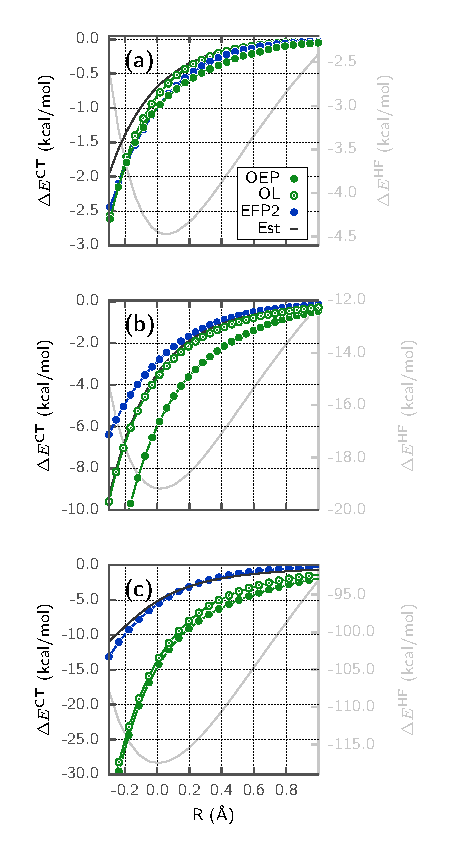
\includegraphics[width=0.5\textwidth]{fig-2.eps}
\caption{\label{f:fig-1} {\bf Accuracy of the OEP approach to estimate the charge transfer energy
in the PT/HF formulation.} 
Asymptotic dependencies of the charge transfer energy is plotted for 
(a) water dimer, 
(b) water\hyp{}ammonium complex, and 
(c) ammonium\hyp{}nitrate complex,
where one molecule has been translated by $R$ from the starting geometry
along the vector specified in Fig. 1.
The counterpoise\hyp{}corrected total interaction energy
is also shown for comparison in light grey color in this figure.
All data were obtained at HF/6-31+G** level of theory.
} 
\end{figure}
%


\subsection{\label{s:413s6}Reduction of computational costs}

The utmost goal of this work is to reduce the computational cost of
the CT PT/HF energy evaluation in the calculations involving effective fragment
potentials. The EFP2 CT expression has the computational cost
roughly proportional to $(10on^2 + 2n^3 + o^2n^2)v$, where the
$o$ and $n$ denote the number of occupied orbitals and the number of atomic basis functions,
respectively, whereas $v$ is the relative cost. On the other hand, OEP\hyp{}based expression
from Eq.~\eqref{} has the cost of approximately $on(Q+N+o)$, where 
$Q$ and $N$ denote the number of auxiliary basis functions and the number of atoms,
respectively. 

In this section, computational cost is estimated from the formulas.
In
Table~\ref{t:oep-costs} 
%
{
\renewcommand{\arraystretch}{1.4}
\begin{table}[b]
\caption[Computational cost of the benchmark and OEP-based methods: calculation of coupling constant]
{{\bf Computational cost of the benchmark and OEP-based methods\footnotemark[1]}
}
\label{t:oep-costs}
\begin{ruledtabular}
\begin{tabular}{lcccccc}
Method             && Murrell et al. &&    EFP2        &&      OEP     \\ 
	\cline{1-7}
Group (i)         &&  &&        &&   $obQ$     \\
Group (ii)        &&  &&        &&   $ob$      \\
Group (iii)       &&  &&        &&   $ob(n+o)$     \\
Total Cost        &&  && $10ob^2 + 2b^3 + o^2b^2$       &&   $ob(Q+n+o)$     \\
\end{tabular}
\end{ruledtabular}
%
\footnotetext[1]{Numbers of: $o$ - occupied molecular orbitals; $b$ - atomic basis functions; $n$ - atoms; 
$Q$ - auxiliary basis functions. It was assumed that the number of virtual orbitals is equal to $b$.}
%
\end{table}
}
%
It is clear that the cost of the OEP\hyp{}based equations is much lesser than the cost of EFP2 method,
and many orders of magnitude lesser than the original theory of Murrell et al.


\section{\label{s:6}Summary and a few concluding remarks}

Bla.

\begin{acknowledgments}
This project is carried out under POLONEZ programme which has received funding from the European Union's
Horizon~2020 research and innovation programme under the Marie Skłodowska-Curie grant agreement 
No.~665778. This project is funded by National Science Centre, Poland 
(grant~no. 2016/23/P/ST4/01720) within the POLONEZ 3 fellowship.
\end{acknowledgments}

%%
\appendix

\section{Optimized Auxiliary Basis Sets for OEP Applications\label{a:auxiliary-basis}}

To fit the auxiliary DF basis for the treatment of the overlap\hyp{}like
OEP matrix elements with the operator $\hat{v}_{\rm eff}$, 
the following objective function is minimized
%
\begin{equation} \label{e:a1-obj}
 Z[\{\xi\}] = \sum_{\alpha i} \left[ 
     \tBraKet{\alpha}{\hat{v}_{\rm eff}}{i} - 
     \sum_{\xi}^{\rm DF} V_{\xi i} S_{\alpha \xi} 
    \right]^2 \;,
\end{equation}
%
where $\{\xi\}$ is the auxiliary basis set to optimize, whereas $\{\alpha\}$
is the `test' basis set used to probe the accuracy of the density fitting.
The forms of the Pauli and charge\hyp{}transfer DF matrices $\tBraKet{\alpha}{\hat{v}_{\rm eff}}{i}$
can be directly derived from Eqs.~\eqref{e:v-oep.rep} and \eqref{e:v-oep.ct}, respectively, 
by expanding the MO's in terms of atomic basis functions. The working formulae
are given below:
%
\begin{subequations} \label{e:a1-v.oep}
 \begin{align}
   \tBraKet{\alpha}{\hat{v}_{\rm eff}^{\rm Rep}}{i}
     &= \sum_{x}^{\rm At} W_{\alpha i}^{(x)} \nonumber   \\ 
        + \sum_{\beta\gamma\delta} &
           \left\{ 
             2 C_{\beta i} D_{\gamma\delta} - C_{\gamma i} D_{\beta \delta}
           \right\}
           \BraKet{\alpha\beta}{\gamma\delta} \;,\\
   \tBraKet{\alpha}{\hat{v}_{\rm eff}^{\rm CT}}{n} 
     &= \sum_{x}^{\rm At} W_{\alpha n}^{(x)} \nonumber   \\
       + \sum_{\beta\gamma\delta} &
           \left\{
             2 C_{\beta n} D_{\gamma\delta} - C_{\gamma n} D_{\beta \delta}
           \right\}
           \BraKet{\alpha\beta}{\gamma\delta}
    \;.
 \end{align}
\end{subequations}
%
In the above equations, ${\bf C}$ is the LCAO\hyp{}MO matrix whereas ${\bf D}$
is the one\hyp{}particle density matrix in AO basis.

%
%\section{\label{a:mcmurchie-davidson} McMurchie-Davidson Method for Asymmetric Electron Repulsion Integrals}
%
%Evaluation of integrals $(ijk\vert l)$,
%that are necessary for the generalized density fitting of OEP's,
%can be easily carried out by re\hyp{}expressing the
%unnormalized product of three primitive Gaussian\hyp{}type (GTO) functions,
%%
%\begin{equation} \label{e:1}
%[ijk] \equiv \phi_i({\bf r}) \phi_j({\bf r}) \phi_k({\bf r}) \;,
%\end{equation}
%%
%in terms of Hermite functions. It can be shown that
%%
%\begin{multline} \label{e:2}
%   [ijk] = E_{ijk} \sum_{N=0}^{n_1+n_2+n_3} \sum_{L=0}^{l_1+l_2+l+3} \sum_{M=0}^{m_1+m_2+m_3} 
%	\\
%          d_N^{n_1n_2n_3} d_L^{l_1l_2l_3} d_M^{m_1m_2m_3}
%          \Lambda_N(x_R)\Lambda_L(y_R)\Lambda_M(z_R)e^{-\alpha_Rr_R^2}
%\end{multline}
%%
%in which the McMurchie-Davidson $d3$ coefficients are given by the following recurrence relationships
%%
% \begin{align} \label{e:3}
%  d_N^{n_1+1,n_2,n_3} &= \frac{1}{2\alpha_R} d_{N-1}^{n_1n_2n_3} 
%                             + \vert {\bf R} - {\bf A}\vert_x d_N^{n_1n_2n_3} \nonumber \\ 
%			    & \qquad\qquad + (N+1) d_{N+1}^{n_1n_2n_3} \\
%  d_N^{n_1,n_2+1,n_3} &= \frac{1}{2\alpha_R} d_{N-1}^{n_1n_2n_3} 
%                             + \vert {\bf R} - {\bf B}\vert_x d_N^{n_1n_2n_3} \nonumber \\
%			    & \qquad\qquad + (N+1) d_{N+1}^{n_1n_2n_3} \\
%  d_N^{n_1,n_2,n_3+1} &= \frac{1}{2\alpha_R} d_{N-1}^{n_1n_2n_3} 
%                             + \vert {\bf R} - {\bf C}\vert_x d_N^{n_1n_2n_3} \nonumber \\
%			    & \qquad\qquad + (N+1) d_{N+1}^{n_1n_2n_3} 
%\end{align}
%%
%with $d_0^{000} = 1$.
%In Eq.~\eqref{e:1},
%$\phi_i({\bf r})$ is given by
%%
%\begin{equation}
%\phi_i({\bf r}) \equiv x_A^{n_1} y_A^{l_1} z_A^{m_1} e^{-\alpha_1r_A^2}
%\end{equation}
%%
%where 
%${\bf r}_A \equiv {\bf r} - {\bf A}$,
%${\bf A}$ is the centre of the GTO, $\alpha_1$ its exponent, whereas $n_1,l_1,m_1$
%the Cartesian angular momenta, with the total angular momentum $\theta_1 = n_1+l_1+m_1$.
%
%It can be easily shown that the multiplicative constant $E_{ijk}$ is given by
%%
%\begin{multline}
%  E_{ijk}(\alpha_1,\alpha_2,\alpha_3)  = \exp{\left[-\frac{\alpha_1\alpha_2}
%                                        {\alpha_1+\alpha_2}\vert {\bf A}-{\bf B}\vert^2\right]} \\ \times
%                                         \exp{\left[-\frac{(\alpha_1+\alpha_2)\alpha_3}
%                                        {\alpha_1+\alpha_2+\alpha_3}
%                                         \vert {\bf P}-{\bf C}\vert^2\right]} 
%\end{multline}
%%

% -----------------------
\bibliography{references}
% -----------------------

\end{document}
